\section{Trend analysis}
0. Data Preprocessing
1. Data Format
As described in the READ.ME of data provided, The targeted data is from the Korean Herald, National Section news. The period of the dataset is from 2015 to 2017. The Crawled date of the dataset is 2018-10-26. Data format is Json, and there are total of 6 data headers - title, author, time, description, body, and section. Total of 23769 news are included in this dataset.
2. Load Data
In order to load the data, the instructions recommended at READ.ME are followed. Pandas library is used for better storing and access of the news text.
3. Libraries Used
For this project, we used pandas and gensim python libraries.


1.
Experiments
0. Idea
0-0. Main idea and Previous approaches
Issue trend analysis can be seen as a part of Topic modeling. By searching fields of recent Topic modeling, LDA has shown to have good performance. As a result, LDA is used as a baseline algorithm for this project.
A recent study(2018) on Topic Modeling shows that Topic Quality improves when Named Entities are promoted.[ref: https://www.aclweb.org/anthology/P18-2040.pdf] This paper proposes 2 techniques: 1)Independent Named Entity Promoting and 2)Document Dependent Named Entity Promoting. Independent Named Entity Promoting promotes the importance of the named entities by applying scalar multiplication alpha to the importance of the named entity word. Document Dependent Named Entity Promoting promotes the importance of the named entities by setting the weights of the named entities as maximum term-frequency per document. For Independent Named Entity Promoting, the value of alpha can be changed flexibily, but results conducted by this paper shows that setting alpha as 10 showed the best results.
We take advantage of this paper and implement Named Entity Promoted Topic Modeling done by LDA.

1. Data Tokenization
1-1. Lemmatization is not always good
At first try, Lemmatization(converting words into base forms) and removal of stopwords were conducted before we run the LDA algorithm and extract Named Entities. We thought that converting words into base forms and reducing the total vocabulary size would increase the performance of topic modeling. Stopwords were taken from nltk.corpus.stopwords.words("english"), and lemmatization function was taken from gensim.utils.lemmatize. ```res.append(lemmatize(raw_text, stopwords=stopwords))``` But after we do lemmatization, remove stopwords, and tokenize the data, no Named Entities were extracted from the preprocessed corpus. We think the reason for this is as follows. 
First, words are all converted into lower case when we do lemmatization. This makes the Named Entitiy Recognition system(NER system) to work poorly because we have removed the original information whether the word has a high probability that it is a "Proper pronoun" or not.(goyue daemeoung sa).
Second, words are transformed into their base forms, limiting NER system to detect specific words. There also could be cases that the words are transformed into meanings other then their original meanings. For example, "Cooking" and "Cooker" are both converted into "cook" when they are lemmatized, and this makes the word to lose the original information.
Third, original relationships between words are lost, because of the removal of stopwords. When we do NER, we have to do the POS tagging of the sentence and then input both the word sequence and the POS sequence of the text. But when we artificially remove stopwords and then do NER, original relationships between words are disrupted and broken. This limits NER system to perform well.

For these 3 reasons, we decided to NOT apply lemmatization for tokenization, because lemmatization lose so much information about the original text and disrupts the NER system's ability to detect Named Entities properly. We decided to just do POS tagging and then do NER. We just used word_tokenize from nltk.tokenize.

2. Extract NER
By using ne_chunk from nltk and pos_tag from nltk.tag, we extracted Named entities from the original news dataset. NER also extracts multi-word information of Named Entities other than just classifying whether a word is a named entity or not, so we decided to use that information. We store single-word Named Entities and multi-word named entities separately. As a result, NER and multi-word extraction of NER are both processed.

below figure is the topic modeling result(of all time lengths from 2015 to 2017) WITH NER Promoting and WITHOUT NER Promoting. We can see the difference between those two results, and we can conclude topic modeling with NER promoting shows better performance.
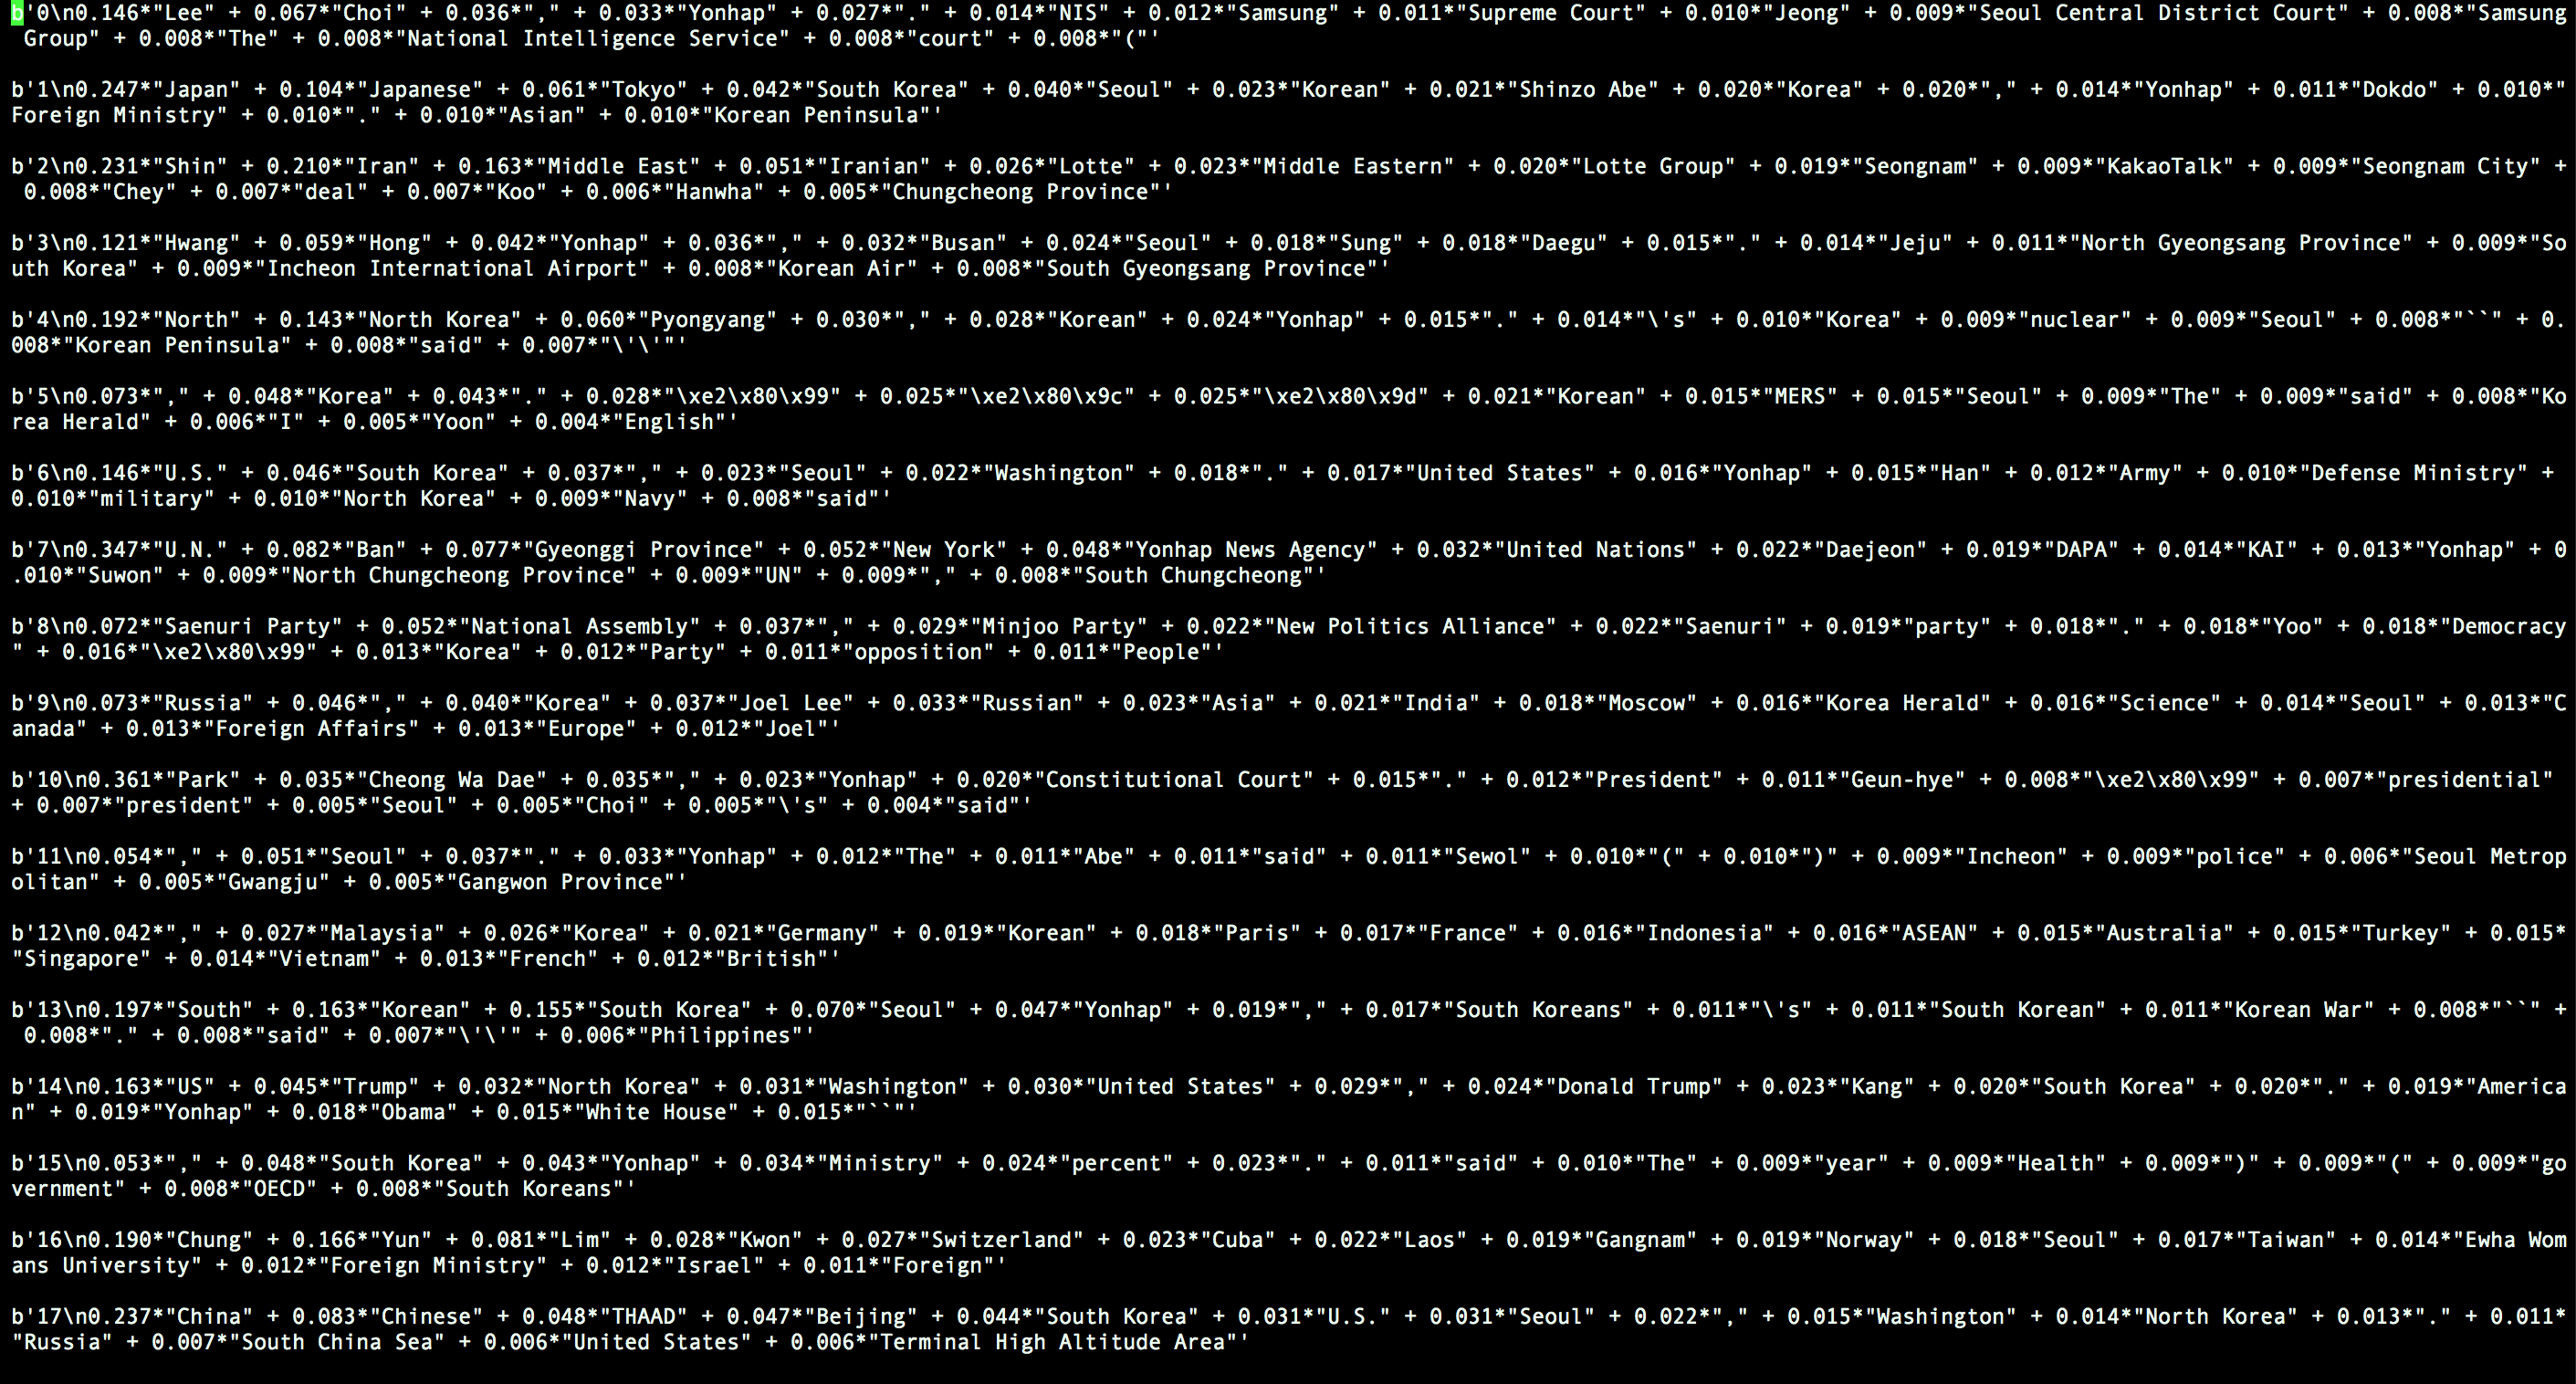
\includegraphics[scale= 0.4]{after_ner.png}
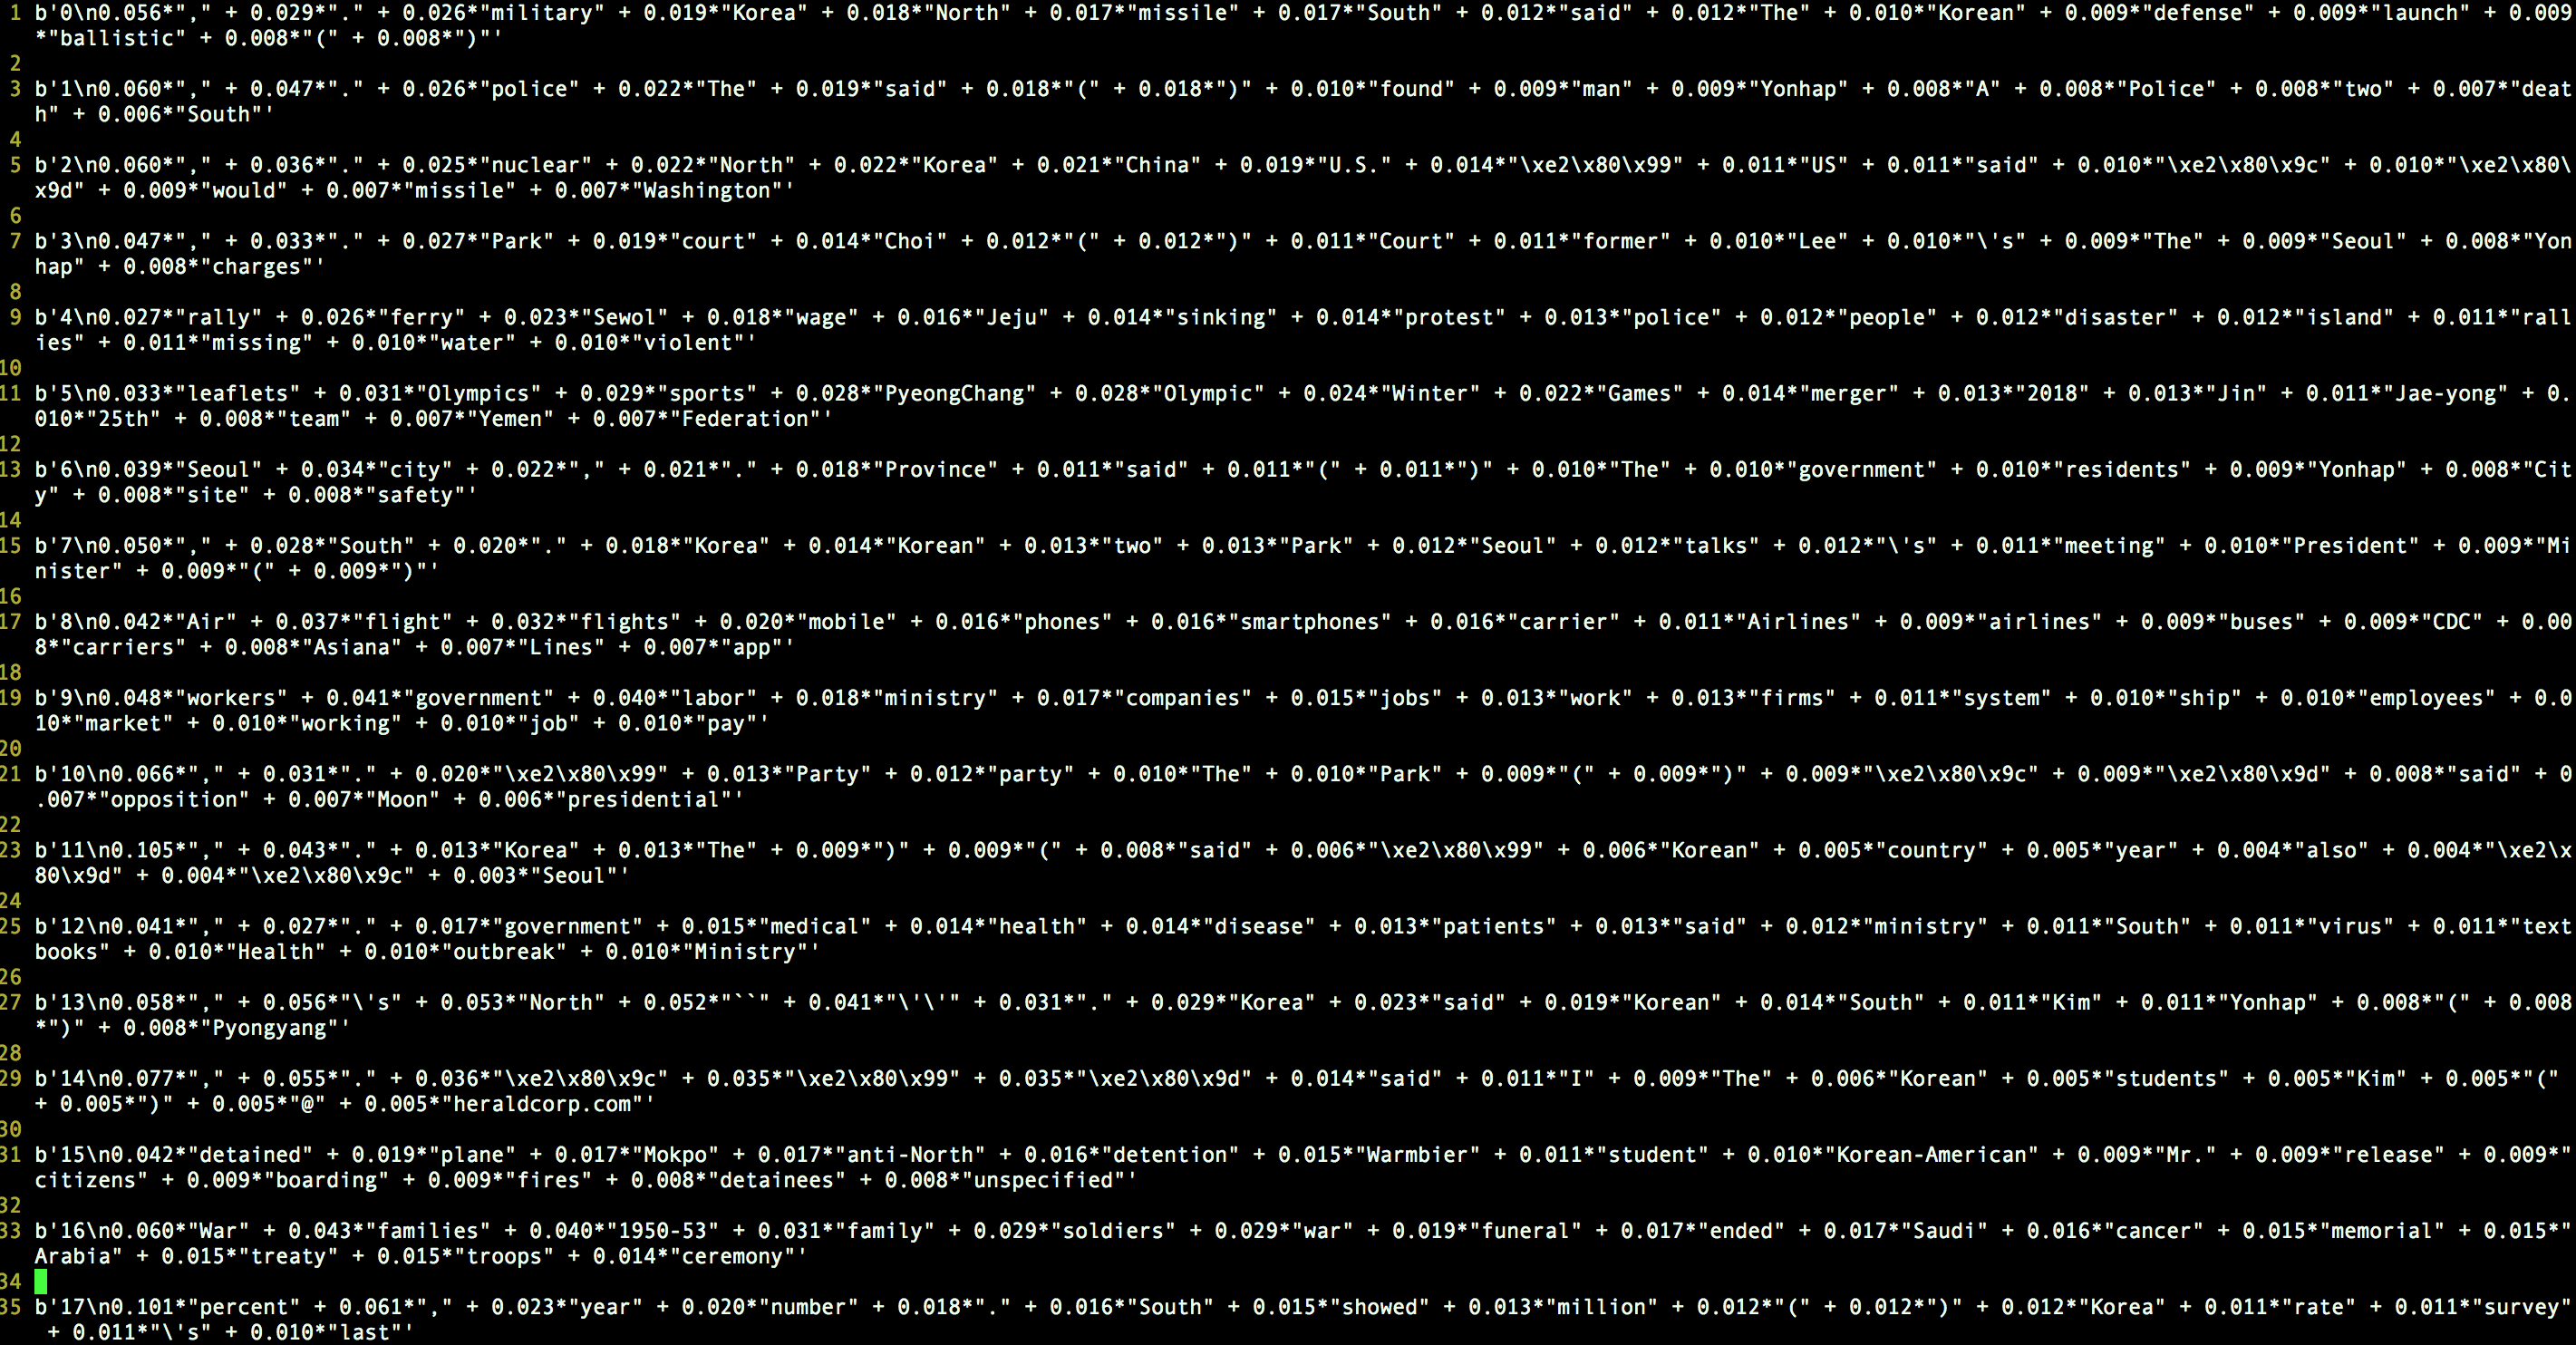
\includegraphics[scale= 0.4]{before_ner.png}
3. Do LDA
At first try, we ran LDA ~~.
But we found out that stopwords are classified as top(important)words according to the result of LDA. So we decided to remove stopwords AFTER all the preprocssing(including NER weight promoting)were done. (The timing of removal of stopwords are important!) After the removal of stopwords, we could see that the result were much better. (Need to include graphics or charts)
